\chapter{\ifproject%
\ifenglish Project Structure and Methodology\else โครงสร้างและขั้นตอนการทำงาน\fi
\else%
\ifenglish Project Structure\else โครงสร้างของโครงงาน\fi
\fi
}

\makeatletter

% \renewcommand\section{\@startsection {section}{1}{\z@}%
%                                    {13.5ex \@plus -1ex \@minus -.2ex}%
%                                    {2.3ex \@plus.2ex}%
%                                    {\normalfont\large\bfseries}}

\makeatother
%\vspace{2ex}
% \titleformat{\section}{\normalfont\bfseries}{\thesection}{1em}{}
% \titlespacing*{\section}{0pt}{10ex}{0pt}

\section{การออกแบบ}

\subsection{Ansible}
\hspace{0.5in} Ansible เป็น Open Source Software Automation Tool ที่ใช้ YAML syntax ในการเขียน Playbook เพื่อทำการตั้งค่าอุปกรณ์เครือข่าย ข้อดีของการใช้ Ansible ในการออกแบบมีดังนี้ 
\begin{itemize}
  \item ใช้งานง่าย: Ansible เขียนด้วย YAML syntax เข้าใจง่าย
  \item Agentless: ไม่จำเป็นต้องติดตั้ง agent บนเครื่อง Remote
  \item Powerful: รองรับการ Automation งานต่างๆ มากมาย
  \item Flexible: รองรับระบบปฏิบัติการหลายประเภท
\end{itemize}
\hspace{0.5in} แต่การใช้งานเพียงแค่ Ansible สำหรับการตั้งค่าเครือข่ายนั้นมีความค่อนข้างยุ่งยากเนื่องจากต้องทำงานผ่าน CLIs ซึ่งอาจเป็นเรื่องยากสำหรับผู้ใช้บางคน

\subsection{Ansible AWX}
\hspace{0.5in} Ansible AWX เป็น Open Source Web Application ที่ช่วยจัดการ Workflow ของ Ansible โดยสั่งผ่าน GUI ดังนั้นโครงงานนี้จึงเลือกที่จะใช้ Ansible AWX เป็น GUI สำหรับควบตุมการทำงานของ Ansible ซึ่งข้อดีของการใช้ Ansible AWX ในการจัดการอุปกรณ์เครือข่าย มีดังนี้
\begin{itemize}
  \item Centralized Management: ควบคุมจัดการ Jobs, Playbooks, Inventory และ Credentials ทั้งหมดจากจุดเดียว
  \item Role-Based Access Control: กำหนดสิทธิ์การเข้าถึงสำหรับผู้ใช้แต่ละคน
  \item Integrations: รองรับการผสานรวมกับ Tools อื่นๆ เช่น Jenkins, GitLab และ GitHub
  \item Notification: มีการแจ้งเตือนผู้ใช้เมื่อมี Errors เกิดขึ้น
\end{itemize}
\hspace{0.5in} การใช้ Ansible AWX ใน Web Application สำหรับ Automation จะช่วยติดตามสถานะการทำงาน จัดการกลุ่มเป้าหมาย (Inventory) ค้นหาและดูข้อมูลย้อนหลัง และสามารถตรวจสอบปัญหาต่างๆที่เกิดขึ้นในเมื่อเกิด Errors

\subsection{Web Application}
\hspace{0.5in} เนื่องจากการใช้งาน Ansible AWX นั้นมีข้อดีที่สามารถเข้าไปจัดการตั้งค่าอุปกรณ์ได้ทีละหลายอุปกรณ์ แต่ยังมีข้อจำกัดคือ ไม่สามารถเช็คความถูกต้องว่าผู้ใช้งานตั้งค่าอุปกรณ์เครือข่ายจากการรัน Templates บน Ansible AWX แล้วอุปกรณ์เครือข่ายนั้นทำงานได้ถูกต้องจริงหรือไม่ จึงทำการออกแบบ Web Application ที่มีระบบตรวจสอบความถูกต้อง และใช้ AWX REST API ในการดึงข้อมูลของอุปกรณ์เครือข่ายทำที่ได้ทำการตั้งค่าไว้ มาคำนวณกับระบบตรวจสอบความถูกต้องใน Web Application เพื่อยืนยันว่าการทำงานของอุปกรณ์เครือข่ายตรงกับที่ผู้ใช้ต้องการตั้งค่า โดยที่ตัว Web Application จะเป็นหน้าหลักสำหรับการใช้งานของผู้ใช้ โดยที่จะทำการตั้งค่าและตรวจสอบอุปกรณ์เครือข่ายผ่าน Web Application
\subsection{ชุดคำสั่งเครือข่ายที่นำมาใช้กับระบบ}
\hspace{0.5in} ในระบบนี้ได้แบ่งการตั้งค่าและการตรวจสอบการตั้งค่า ออกเป็น 2 ส่วนคือ ส่วนของ Switch และส่วนของ Router โดยได้นำไฟล์ Playbooks ที่ผู้พัฒนาได้จัดทำไว้เพื่อมาสร้างเป็น Templates สำหรับการทำงาน โดยจะมีบาง Templates โดยชุดคำสั่งการตั้งค่าและการตรวจสอบการตั้งค่าที่เลือกมานั้น เพียงพอต่อการตั้งค่าและการตรวจสอบการตั้งค่าเครือข่ายพื้นฐาน โดยที่ชุดคำสั่งมีดังนี้
\begin{itemize}
  \item Router:
  \begin{itemize}
    \item Device Name
    \item Interface status
    \item Interface IP address
    \item Static route
    \item Default route
    \item RIP
    \item OSPF
  \end{itemize}
  \item Switch:
  \begin{itemize}
    \item Device Name
    \item Interface status
    \item Interface switchport
    \item VLAN
    \item VTP mode \& domain 
    \item VTP password
    \item Default gateway
    \item Spanning-tree priority
  \end{itemize}
\end{itemize}
\section{โครงสร้างการทำงาน}
\hspace{0.5in} การทำงานของ Web Application จะเป็นการใช้ AWX API มาแสดงผลบน Web Application ที่สร้างขึ้นมาโดยจะมีฟังก์ชันหลักๆดังนี้
\begin{itemize}
  \item Configuration: ผู้ใช้สามารถเลือก Templates ที่ต้องการผ่าน Web Application โดยไม่จำเป็นต้องสร้าง Templates ขึ้นมาเองเนื่องจาก Templates นั้นถูกสร้างแบบสำเร็จรูปไว้เรียบร้อยแล้วใน Ansible AWX โดยผู้ใช้จะทำเพียงแค่เลือก Templates ที่ผู้ใช้ต้องการจัดการและกรอกข้อมูล Hosts และ Configuration ต่างๆใน Web Application จากนั้น Web Application จะนำข้อมูลที่ผู้ใช้กรอกส่งไปยัง Ansible AWX เพื่อให้ Ansible AWX รับคำสั่งและทำตามคำสั่งเหล่านั้นในอุปกรณ์เน็ตเวิร์คที่ผู้ใช้ได้กำหนดไว้
  \item Verification: ผู้ใช้สามารถตรวจสอบความถูกต้องได้จาก Templates ประเภท Verification ได้ ผ่าน Web Application ซึ่งจะตรวจสอบโดยใช้ Verify Configuration Commmands ต่างๆ เช่น show running-config, show vlan, show startup-config หรือ show interfaces เป็นต้น โดยคำสั่งเหล่านี้จะถูกเรียกใช้บน Ansible AWX ที่จะรับคำสั่งมาจาก Web Application นั้นอีกที ออกมาเป็นไฟล์ประเภท json ซึ่งจะนำมา filter เฉพาะส่วนที่ต้องการ และเปรียบเทียบความถูกต้องกับไฟล์ json ของ Web Application ซึ่งไฟล์ json ของ Web Application ไม่ได้เรียกใช้ Verify Configuration Commmands โดยตรง แต่จะได้จากระบบตรวจสอบความถูกต้องจาก Web Application ที่โปรแกรมขึั้นมาเอง
\end{itemize}

รูปที่ \ref{fig:api} แสดงโครงสร้างการทำงาน ของ Web Application

\begin{figure}[h]
  \begin{center}
    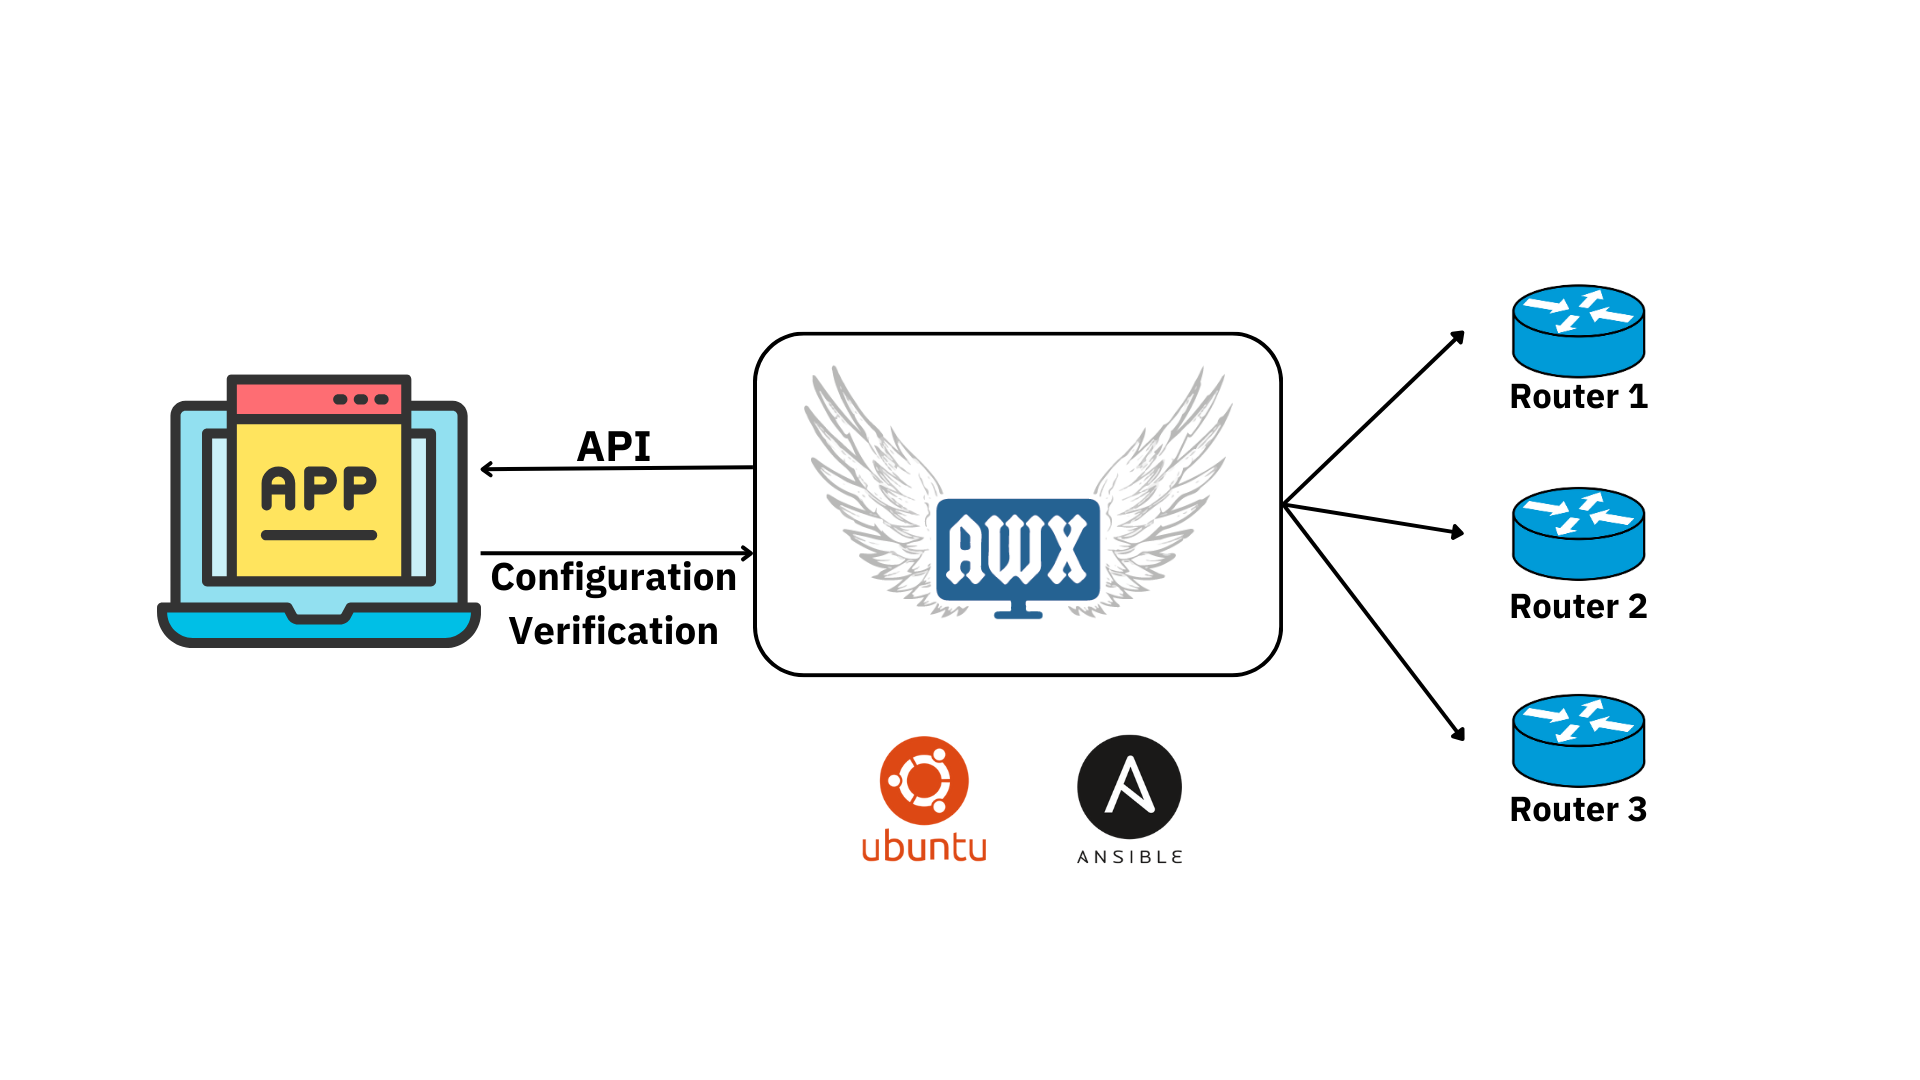
\includegraphics[scale=0.25]{API.png}
  \end{center}
  \caption[โครงการทำงานของ Web Application ที่ออกแบบไว้เบื้องต้น]{โครงการทำงานของ Web Application ที่ออกแบบไว้เบื้องต้น}
  \label{fig:api}
\end{figure}